\documentclass{article}\usepackage[]{graphicx}\usepackage[]{color}
%% maxwidth is the original width if it is less than linewidth
%% otherwise use linewidth (to make sure the graphics do not exceed the margin)
\makeatletter
\def\maxwidth{ %
  \ifdim\Gin@nat@width>\linewidth
    \linewidth
  \else
    \Gin@nat@width
  \fi
}
\makeatother

\definecolor{fgcolor}{rgb}{0.514, 0.58, 0.588}
\newcommand{\hlnum}[1]{\textcolor[rgb]{0.863,0.196,0.184}{#1}}%
\newcommand{\hlstr}[1]{\textcolor[rgb]{0.863,0.196,0.184}{#1}}%
\newcommand{\hlcom}[1]{\textcolor[rgb]{0.345,0.431,0.459}{#1}}%
\newcommand{\hlopt}[1]{\textcolor[rgb]{0.576,0.631,0.631}{#1}}%
\newcommand{\hlstd}[1]{\textcolor[rgb]{0.514,0.58,0.588}{#1}}%
\newcommand{\hlkwa}[1]{\textcolor[rgb]{0.796,0.294,0.086}{#1}}%
\newcommand{\hlkwb}[1]{\textcolor[rgb]{0.522,0.6,0}{#1}}%
\newcommand{\hlkwc}[1]{\textcolor[rgb]{0.796,0.294,0.086}{#1}}%
\newcommand{\hlkwd}[1]{\textcolor[rgb]{0.576,0.631,0.631}{#1}}%

\usepackage{framed}
\makeatletter
\newenvironment{kframe}{%
 \def\at@end@of@kframe{}%
 \ifinner\ifhmode%
  \def\at@end@of@kframe{\end{minipage}}%
  \begin{minipage}{\columnwidth}%
 \fi\fi%
 \def\FrameCommand##1{\hskip\@totalleftmargin \hskip-\fboxsep
 \colorbox{shadecolor}{##1}\hskip-\fboxsep
     % There is no \\@totalrightmargin, so:
     \hskip-\linewidth \hskip-\@totalleftmargin \hskip\columnwidth}%
 \MakeFramed {\advance\hsize-\width
   \@totalleftmargin\z@ \linewidth\hsize
   \@setminipage}}%
 {\par\unskip\endMakeFramed%
 \at@end@of@kframe}
\makeatother

\definecolor{shadecolor}{rgb}{.97, .97, .97}
\definecolor{messagecolor}{rgb}{0, 0, 0}
\definecolor{warningcolor}{rgb}{1, 0, 1}
\definecolor{errorcolor}{rgb}{1, 0, 0}
\newenvironment{knitrout}{}{} % an empty environment to be redefined in TeX

\usepackage{alltt}
\usepackage{geometry}
\geometry{verbose, tmargin=2.5cm, bmargin=2.5cm, lmargin=2.5cm, rmargin=2.5cm}
\IfFileExists{upquote.sty}{\usepackage{upquote}}{}
\begin{document}

\title{Data Extraction Evaluation}
\author{Matthew Leonawicz}
\maketitle





\subsection{Next steps}

Combining sampling and data reduction methods while using the most efficient \textbf{R} functions can be particularly useful when processing large numbers of high-resolution geotiff raster layers.
One thing I already do when extracting from many files by shapefile is I avoid extracting by shape more than once.
I do it one time to obtain the corresponding raster layer cell indices.
Then on all subsequent maps I extract by cell indices which is notably faster.
Ultimately, there is much more room for speed improvements in terms of efficient use of statistics than in strictly programmatic corner-cutting.

The plots below benchmark different sample mean computations.
Comparisons involve the sample mean of the entire data set and do not involve the main approach outlined above which focuses on efficiency gains by taking the mean of a smaller, representative sample.
This provides some insight into how it is beneficial nonetheless to considering the right programmatic approach in conjunction with statistical efficiencies.

\begin{knitrout}
\definecolor{shadecolor}{rgb}{0, 0.169, 0.212}\color{fgcolor}\begin{kframe}
\begin{verbatim}
## Unit: milliseconds
##                              expr       min        lq      mean    median
##                mean(v, na.rm = T) 393.64885 394.81215 401.46656 395.44489
##                  mean(v[dat.ind])  13.93193  14.05525  14.87471  14.10687
##                sum(v[dat.ind])/nd  12.44504  12.54393  15.47461  12.59665
##       .Internal(mean(v[dat.ind]))  13.80660  13.98169  15.74200  14.04980
##  .Primitive("sum")(v[dat.ind])/nd  12.43477  12.56648  14.37262  12.61655
##         uq       max neval
##  406.43661 510.61899   100
##   14.16596  37.87314   100
##   12.68451  38.03828   100
##   14.18867  38.37634   100
##   12.67938  38.26842   100
\end{verbatim}
\end{kframe}
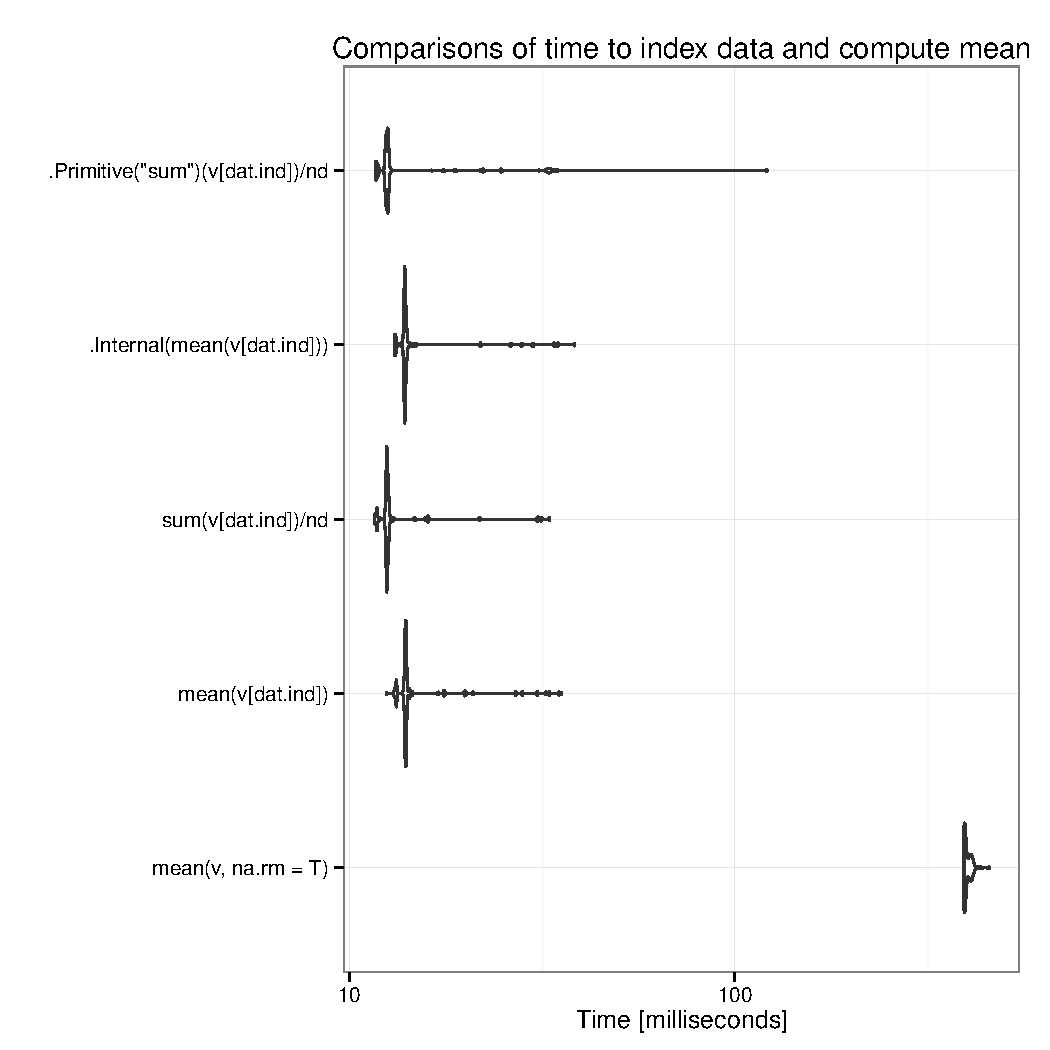
\includegraphics[width=\maxwidth]{figure/benchmarks1-1} 

\end{knitrout}

\begin{knitrout}
\definecolor{shadecolor}{rgb}{0, 0.169, 0.212}\color{fgcolor}\begin{kframe}
\begin{verbatim}
## Unit: milliseconds
##                expr       min        lq      mean    median        uq
##    mean(v[dat.ind]) 13.893058 14.087589 16.219392 14.191308 14.419740
##  sum(v[dat.ind])/nd 12.397452 12.577522 14.224463 12.666780 12.864421
##             mean(d)  2.947051  2.970065  3.041987  2.997433  3.041284
##           sum(d)/nd  1.483478  1.496229  1.528518  1.503382  1.529817
##         max neval
##  129.023621  1000
##   41.267096  1000
##    4.709807  1000
##    3.047504  1000
\end{verbatim}
\end{kframe}
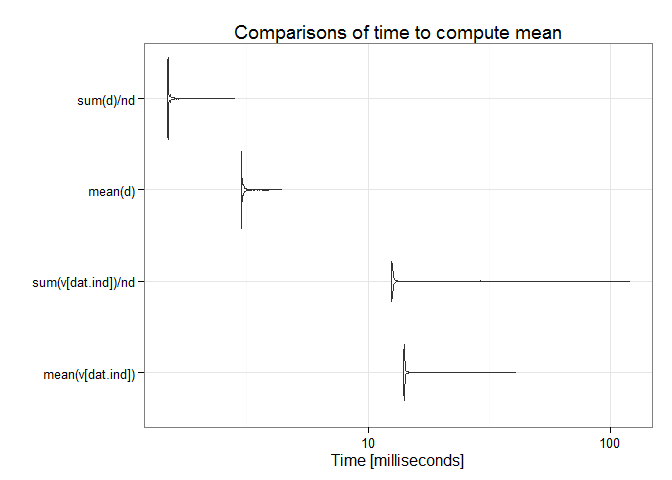
\includegraphics[width=\maxwidth]{figure/benchmarks2-1} 

\end{knitrout}

\end{document}
